\section{Model\-Car\-Dyn\-Smooth\-Rollover  Class Reference}
\label{classModelCarDynSmoothRollover}\index{ModelCarDynSmoothRollover@{Model\-Car\-Dyn\-Smooth\-Rollover}}
One more dimension than {\bf Model\-Car\-Dyn\-Rollover} {\rm (p.\,\pageref{classModelCarDynRollover})} considering the steering angle can only change continuously. 


{\tt \#include $<$modelcar.h$>$}

Inheritance diagram for Model\-Car\-Dyn\-Smooth\-Rollover::\begin{figure}[H]
\begin{center}
\leavevmode
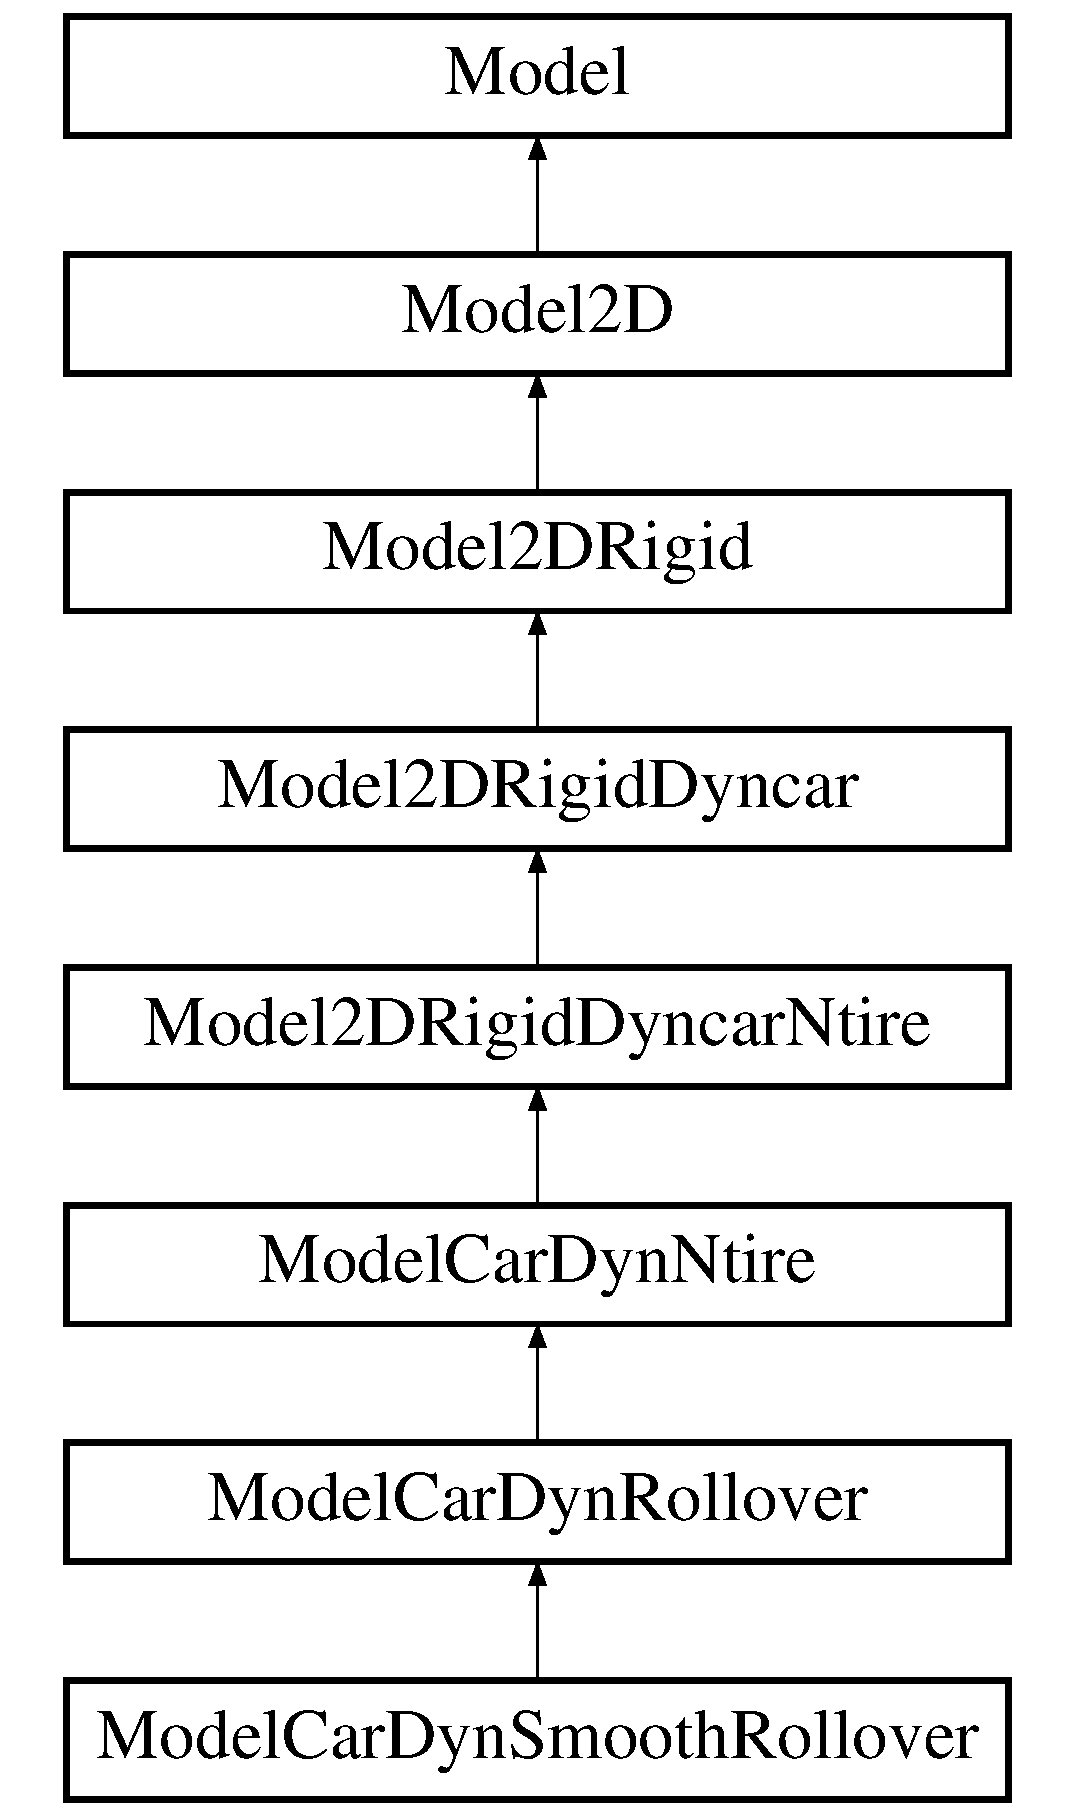
\includegraphics[height=8cm]{classModelCarDynSmoothRollover}
\end{center}
\end{figure}
\subsection*{Public Methods}
\begin{CompactItemize}
\item 
{\bf Model\-Car\-Dyn\-Smooth\-Rollover} (string path)
\item 
virtual {\bf $\sim$Model\-Car\-Dyn\-Smooth\-Rollover} ()
\item 
virtual {\bf MSLVector} {\bf State\-Transition\-Equation} (const {\bf MSLVector} \&x1, const {\bf MSLVector} \&u)
\begin{CompactList}\small\item\em The state transition equation, or equations of motion, xdot=f(x,u).\item\end{CompactList}\item 
virtual {\bf MSLVector} {\bf State\-To\-Configuration} (const {\bf MSLVector} \&{\bf x})
\begin{CompactList}\small\item\em A method that converts a {\bf Model} {\rm (p.\,\pageref{classModel})} state in to a {\bf Geom} {\rm (p.\,\pageref{classGeom})} configuration.\item\end{CompactList}\item 
virtual double {\bf Metric} (const {\bf MSLVector} \&x1, const {\bf MSLVector} \&x2)
\begin{CompactList}\small\item\em A distance metric, which is Euclidean in the base class.\item\end{CompactList}\item 
virtual {\bf MSLVector} {\bf Linear\-Interpolate} (const {\bf MSLVector} \&x1, const {\bf MSLVector} \&x2, const double \&a)
\begin{CompactList}\small\item\em Linearly interpolate two state while respecting topology.\item\end{CompactList}\end{CompactItemize}


\subsection{Detailed Description}
One more dimension than {\bf Model\-Car\-Dyn\-Rollover} {\rm (p.\,\pageref{classModelCarDynRollover})} considering the steering angle can only change continuously.



\subsection{Constructor \& Destructor Documentation}
\index{ModelCarDynSmoothRollover@{Model\-Car\-Dyn\-Smooth\-Rollover}!ModelCarDynSmoothRollover@{ModelCarDynSmoothRollover}}
\index{ModelCarDynSmoothRollover@{ModelCarDynSmoothRollover}!ModelCarDynSmoothRollover@{Model\-Car\-Dyn\-Smooth\-Rollover}}
\subsubsection{\setlength{\rightskip}{0pt plus 5cm}Model\-Car\-Dyn\-Smooth\-Rollover::Model\-Car\-Dyn\-Smooth\-Rollover (string {\em path} = \char`\"{}\char`\"{})}\label{classModelCarDynSmoothRollover_a0}


\index{ModelCarDynSmoothRollover@{Model\-Car\-Dyn\-Smooth\-Rollover}!~ModelCarDynSmoothRollover@{$\sim$ModelCarDynSmoothRollover}}
\index{~ModelCarDynSmoothRollover@{$\sim$ModelCarDynSmoothRollover}!ModelCarDynSmoothRollover@{Model\-Car\-Dyn\-Smooth\-Rollover}}
\subsubsection{\setlength{\rightskip}{0pt plus 5cm}Model\-Car\-Dyn\-Smooth\-Rollover::$\sim$Model\-Car\-Dyn\-Smooth\-Rollover ()\hspace{0.3cm}{\tt  [inline, virtual]}}\label{classModelCarDynSmoothRollover_a1}




\subsection{Member Function Documentation}
\index{ModelCarDynSmoothRollover@{Model\-Car\-Dyn\-Smooth\-Rollover}!LinearInterpolate@{LinearInterpolate}}
\index{LinearInterpolate@{LinearInterpolate}!ModelCarDynSmoothRollover@{Model\-Car\-Dyn\-Smooth\-Rollover}}
\subsubsection{\setlength{\rightskip}{0pt plus 5cm}{\bf MSLVector} Model\-Car\-Dyn\-Smooth\-Rollover::Linear\-Interpolate (const {\bf MSLVector} \& {\em x1}, const {\bf MSLVector} \& {\em x2}, const double \& {\em a})\hspace{0.3cm}{\tt  [virtual]}}\label{classModelCarDynSmoothRollover_a5}


Linearly interpolate two state while respecting topology.

If a=0, then x1 is returned; if a=1, then x2 is returned. All intermediate values of \$a $\backslash$in [0,1]\$ yield intermediate states. This method is defined by {\bf Model} {\rm (p.\,\pageref{classModel})}. 

Reimplemented from {\bf Model2DRigid\-Dyncar} {\rm (p.\,\pageref{classModel2DRigidDyncar_a6})}.\index{ModelCarDynSmoothRollover@{Model\-Car\-Dyn\-Smooth\-Rollover}!Metric@{Metric}}
\index{Metric@{Metric}!ModelCarDynSmoothRollover@{Model\-Car\-Dyn\-Smooth\-Rollover}}
\subsubsection{\setlength{\rightskip}{0pt plus 5cm}double Model\-Car\-Dyn\-Smooth\-Rollover::Metric (const {\bf MSLVector} \& {\em x1}, const {\bf MSLVector} \& {\em x2})\hspace{0.3cm}{\tt  [virtual]}}\label{classModelCarDynSmoothRollover_a4}


A distance metric, which is Euclidean in the base class.



Reimplemented from {\bf Model\-Car\-Dyn\-Rollover} {\rm (p.\,\pageref{classModelCarDynRollover_a6})}.\index{ModelCarDynSmoothRollover@{Model\-Car\-Dyn\-Smooth\-Rollover}!StateToConfiguration@{StateToConfiguration}}
\index{StateToConfiguration@{StateToConfiguration}!ModelCarDynSmoothRollover@{Model\-Car\-Dyn\-Smooth\-Rollover}}
\subsubsection{\setlength{\rightskip}{0pt plus 5cm}{\bf MSLVector} Model\-Car\-Dyn\-Smooth\-Rollover::State\-To\-Configuration (const {\bf MSLVector} \& {\em x})\hspace{0.3cm}{\tt  [virtual]}}\label{classModelCarDynSmoothRollover_a3}


A method that converts a {\bf Model} {\rm (p.\,\pageref{classModel})} state in to a {\bf Geom} {\rm (p.\,\pageref{classGeom})} configuration.



Reimplemented from {\bf Model\-Car\-Dyn\-Rollover} {\rm (p.\,\pageref{classModelCarDynRollover_a4})}.\index{ModelCarDynSmoothRollover@{Model\-Car\-Dyn\-Smooth\-Rollover}!StateTransitionEquation@{StateTransitionEquation}}
\index{StateTransitionEquation@{StateTransitionEquation}!ModelCarDynSmoothRollover@{Model\-Car\-Dyn\-Smooth\-Rollover}}
\subsubsection{\setlength{\rightskip}{0pt plus 5cm}{\bf MSLVector} Model\-Car\-Dyn\-Smooth\-Rollover::State\-Transition\-Equation (const {\bf MSLVector} \& {\em x1}, const {\bf MSLVector} \& {\em u})\hspace{0.3cm}{\tt  [virtual]}}\label{classModelCarDynSmoothRollover_a2}


The state transition equation, or equations of motion, xdot=f(x,u).



Reimplemented from {\bf Model\-Car\-Dyn\-Rollover} {\rm (p.\,\pageref{classModelCarDynRollover_a3})}.

The documentation for this class was generated from the following files:\begin{CompactItemize}
\item 
{\bf modelcar.h}\item 
{\bf modelcar.C}\end{CompactItemize}
